% ============================================================================
%  E-Commerce Purchase Intention Prediction — Project Report
%  Intelligenza Artificiale e Apprendimento Automatico
%  Università degli Studi di Firenze — A.A. 2024/2025
% ============================================================================

\documentclass{article}

% ── Packages ────────────────────────────────────────────────────────────────
\usepackage[utf8]{inputenc}
\usepackage[a4paper,left=3.5cm,right=3.5cm,top=2cm,bottom=2cm]{geometry}
\usepackage{crop,graphicx,amsmath,array,amssymb,fancyhdr,lineno}
\usepackage{flushend,stfloats,amsthm,chngpage,times,lipsum,lastpage}
\usepackage{calc,listings,wrapfig,tabularx,longtable,enumitem}
\usepackage{multirow}
\usepackage{caption}
\usepackage{subcaption}
\usepackage{hyperref}
\usepackage{booktabs}
\usepackage{xcolor}
\usepackage{tcolorbox}
\definecolor{shadecolor}{rgb}{0.86,0.86,0.86}
\usepackage{float}
\usepackage{csquotes}
\usepackage[english]{babel}

\graphicspath{{../Resources/}}

\hypersetup{
    colorlinks=true,
    linkcolor=blue!60!black,
    citecolor=blue!60!black,
    urlcolor=blue!60!black,
}

% ── Header e Footer ────────────────────────────────────────────────────────
\pagestyle{fancy}
\fancypagestyle{plain}{%
  \renewcommand{\headrulewidth}{0pt}%
  \fancyhf{}%
}

\title{E-Commerce Purchase Intention Prediction}
\author{Davide Meta}

% ============================================================================
\begin{document}
\begin{titlepage}
\centering

\includegraphics[width=0.5\textwidth]{firenze2.png}\par\vspace{1cm}
\vspace{2cm}
{\scshape\LARGE UNIVERSITÀ DEGLI STUDI DI FIRENZE \par}
\vspace{1cm}
{\scshape\Large DIPARTIMENTO DI INGEGNERIA DELL'INFORMAZIONE\par}
\vspace{1.5cm}
{\huge\bfseries A Comparative Analysis of Linear and Non-Linear Models for E-Commerce Purchase Prediction\par}
\vspace{2cm}
{\Large\itshape Davide Meta\par}
\vspace{0.5cm}
{\large Student ID: 7136156\par}
\vfill
{\large Main Course:\par}
{\Large\bfseries Intelligenza Artificiale e Apprendimento Automatico\par}
\vspace{0.5cm}
{\large Course Instructor:\par}
{\Large Prof. Federico Pernici\par}
\vfill
\end{titlepage}


\fancyhf{}
\fancyhead[L]{Davide Meta}
\fancyhead[R]{Intelligenza Artificiale e Apprendimento Automatico}
\fancyfoot[R]{ \large \bf \thepage\ \centering}%

\newpage
\tableofcontents
\listoffigures
\listoftables

\newpage
\section{Introduction}

\subsection{Problem Description}

Predicting whether a browsing session on an e-commerce platform will result in a purchase is a highly relevant task for both industry and academia. This work frames the problem as a \textbf{binary classification} task. Given a set of session-level features, the primary goal is to determine whether the user journey ends with a successful transaction (\texttt{Revenue = True}) or an abandonment (\texttt{Revenue = False}). To provide a comprehensive analysis, three distinct learning paradigms are compared:

\begin{itemize}
    \item \textbf{Logistic Regression}: a classic linear model that serves as a highly interpretable baseline.
    \item \textbf{Artificial Neural Networks (ANNs)}: a feedforward architecture capable of capturing complex, non-linear feature interactions.
    \item \textbf{Random Forests}: an ensemble approach consisting of 500 decision trees, enhanced by SHAP-based interpretability.
\end{itemize}

\subsection{Theoretical Background and Metrics}

When dealing with imbalanced classification, relying solely on global accuracy can be highly misleading. A naive baseline simply predicting the majority class would achieve approximately 84.5\% accuracy without learning any underlying pattern. To ensure a robust and fair assessment, the evaluation framework includes:

\begin{itemize}
    \item \textbf{ROC-AUC}: which measures the discriminative ability of the models across all possible classification thresholds.
    \item \textbf{Precision}: the ratio of correctly predicted purchases to all predicted purchases. It evaluates the model's ability to minimize \textit{false positives} (e.g., predicting a purchase when the user actually abandons the cart).
    \item \textbf{Recall (Sensitivity)}: the ratio of correctly predicted purchases to all actual purchases. It evaluates the model's ability to minimize \textit{false negatives} (e.g., failing to identify a user who is going to buy).
    \item \textbf{F1-Score}: the harmonic mean of Precision and Recall. It provides a single, balanced metric that is particularly useful for highly imbalanced datasets where accuracy is misleading.
    \item \textbf{Confusion Matrix}: providing a detailed visual breakdown of prediction errors.
    \item \textbf{SHAP values}~\cite{lundberg2017}: an advanced interpretability method used to quantify the exact contribution of each feature to the model's predictions. It is preferred over traditional Gini-based importance because it consistently shows both the magnitude and the direction of a feature's impact on the final output.
\end{itemize}

From a theoretical standpoint, \textbf{Logistic Regression} models the log-odds of the positive class as a linear combination of features. Moving beyond linear boundaries, \textbf{ANNs}~\cite{goodfellow2016} approximate arbitrary functions through successive compositions of affine transformations and non-linear activations. In this study, the \textbf{ReLU} function ($\max(0, x)$) is employed in the hidden layers to explicitly mitigate the vanishing gradient problem often caused by standard sigmoid activations. Finally, \textbf{Random Forests}~\cite{breiman2001} leverage bootstrap aggregation to combine predictions from multiple decorrelated decision trees, naturally handling non-linearities while resisting overfitting.

\subsection{Exploratory Data Analysis}

The \textit{Online Shoppers Purchasing Intention Dataset}~\cite{sakar2019} from the UCI Machine Learning Repository contains \textbf{12,330 sessions} described by \textbf{18 features}. These comprise 10 numerical variables (such as page-visit counts, durations, bounce and exit rates, alongside page values) and 8 categorical attributes (including month, OS, browser, region, traffic type, visitor type, and weekend status). The Exploratory Data Analysis %(notebook \texttt{01\_eda.ipynb})
highlighted the following main insights:

\begin{itemize}
    \item A \textbf{severe class imbalance}, with 84.5\% non-purchasing sessions versus 15.5\% purchasing sessions (representing a ratio of approximately $5.5:1$).
    \item An excellent data quality, with \textbf{no missing values} across all the 12,330 recorded sessions.
    \item \textbf{PageValues} (a Google Analytics metric representing the average value of a web page visited before a transaction) emerged as the strongest single discriminator for positive purchase behaviour.
    \item \textbf{BounceRates} and \textbf{ExitRates} showed a strong negative correlation with successful transactions.
    \item \textbf{ProductRelated} pages accounted for the vast majority of the total session time.
\end{itemize}

\noindent The full source code, notebooks, and preprocessed data are publicly available on \href{https://github.com/davidemeta/Predicting-Online-Shoppers-Purchasing-Intention}{GitHub}.
\section{Experimental Setup}

\subsection{Split Strategy}

To ensure a robust evaluation and prevent performance estimation bias, the dataset was divided using a \textbf{stratified 80/20 partition}. This approach meticulously preserved the original class ratio across both subsets:

\begin{itemize}
    \item \textbf{Training Set (80\%)}: comprising 9,864 samples used for model training. To address the inherent class imbalance discussed previously, this set was subsequently expanded to 16,676 samples via SMOTE oversampling.
    \item \textbf{Test Set (20\%)}: consisting of 2,466 samples that were kept strictly isolated until the final evaluation phase.
\end{itemize}

Furthermore, when training the Artificial Neural Network (ANN), an additional 15\% validation split was extracted dynamically from the training data. This allowed for real-time monitoring of the validation loss, enabling early stopping to prevent overfitting during the training loop.

\subsection{Preprocessing Pipeline}

A rigorous preprocessing pipeline was established to prepare the raw data for modeling while strictly preventing \textit{data leakage} at every stage. The sequential steps were executed as follows:

\begin{enumerate}
    \item \textbf{Feature Encoding}: categorical variables were systematically transformed into numerical representations. Specifically, the \texttt{Month} feature was ordinal-encoded to reflect its natural temporal progression (e.g., Jan=1 \dots Dec=12), \texttt{VisitorType} was label-encoded, and boolean attributes were directly cast to integers.
    \item \textbf{Feature Scaling}: to ensure all variables contributed equally to the learning process, numerical features were standardized. A \texttt{StandardScaler} was fitted exclusively on the training set to compute the mean and variance, and only then applied to transform both the training and test sets.
    \item \textbf{SMOTE Oversampling}~\cite{chawla2002}: the \textit{Synthetic Minority Over-sampling Technique} was applied solely to the training data. This procedure synthesized new examples for the minority class, effectively balancing the training distribution from 8,338 non-purchases and 1,526 purchases to a symmetric 8,338 to 8,338 ratio. The test set was intentionally left untouched to ensure the final evaluation reflected the true, highly imbalanced operational environment.
\end{enumerate}
\newpage
\section{Results}

\subsection{Training}

The learning dynamics of the Artificial Neural Network are illustrated in Figure~\ref{fig:ann_history}, which displays the training history across epochs. Both the training and validation loss exhibit a steady convergence, eventually triggering the EarlyStopping mechanism at epoch 85. The close alignment of these two curves confirms that the model achieved good generalisation, successfully avoiding significant overfitting on the training data.

\begin{figure}[H]
    \centering
    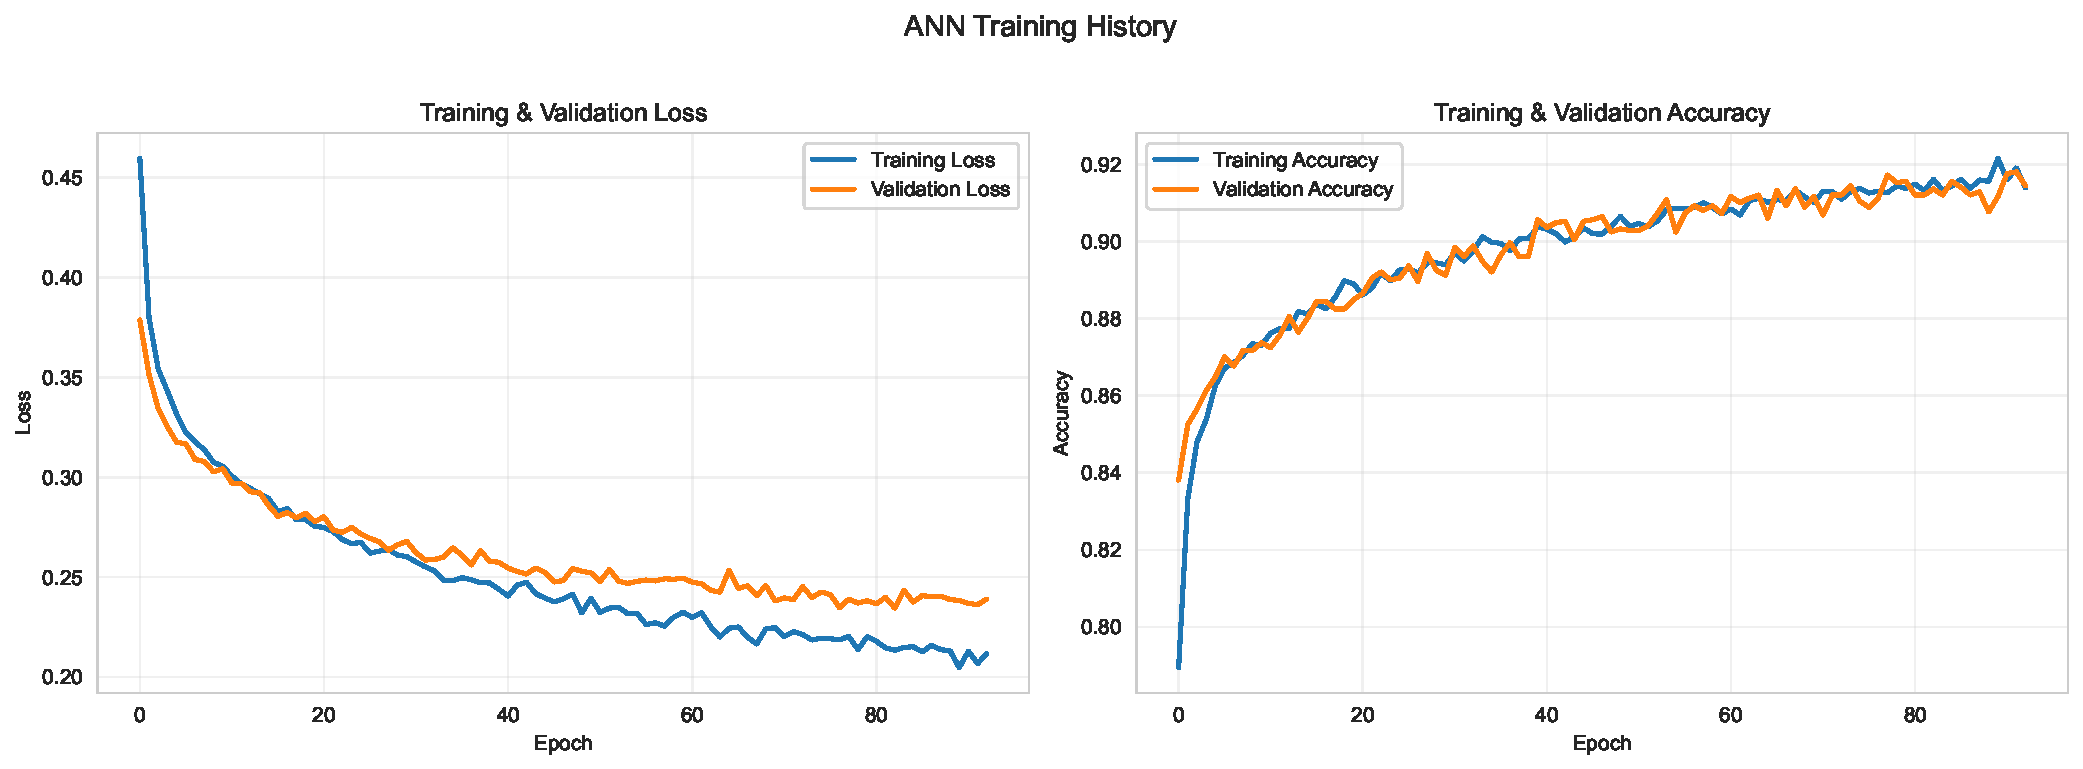
\includegraphics[width=\textwidth]{ann_training_history.pdf}
    \caption{ANN training history: loss (left) and accuracy (right).}
    \label{fig:ann_history}
\end{figure}

\subsection{Comparative Results}

Table~\ref{tab:results} presents a comprehensive summary of the models' performance on the isolated test set. Since predicting the actual transaction is the primary objective of this study, metrics such as Precision, Recall, and the F1-Score are reported specifically for the positive class (purchase).

\begin{table}[H]
\centering
\caption{Test-set performance comparison. Best values per metric in \textbf{bold}.}
\label{tab:results}
\begin{tabular}{@{}lccccc@{}}
\toprule
\textbf{Model} & \textbf{Accuracy} & \textbf{Precision} & \textbf{Recall} & \textbf{F1-Score} & \textbf{ROC-AUC} \\ \midrule
Logistic Regression & 0.8593 & 0.5348 & 0.7042 & 0.6079 & 0.8801 \\
ANN                 & 0.8528 & 0.5174 & \textbf{0.7408} & 0.6093 & 0.8946 \\
Random Forest       & \textbf{0.8897} & \textbf{0.6297} & 0.6990 & \textbf{0.6625} & \textbf{0.9217} \\ \bottomrule
\end{tabular}
\end{table}

These quantitative results are further supported by the comparative ROC curves (Figure~\ref{fig:roc_comp}). The Random Forest model clearly dominates the upper-left region across virtually all classification thresholds, achieving the highest overall ROC-AUC. It is followed by the ANN and the Logistic Regression baseline. 

Furthermore, an analysis of the confusion matrices (Figure~\ref{fig:cm_comp}) reveals distinct behavioural differences among the models. While the Random Forest excels in precision by producing the fewest false positives, the ANN proves to be more sensitive, yielding the fewest false negatives.

\begin{figure}[H]
    \centering
    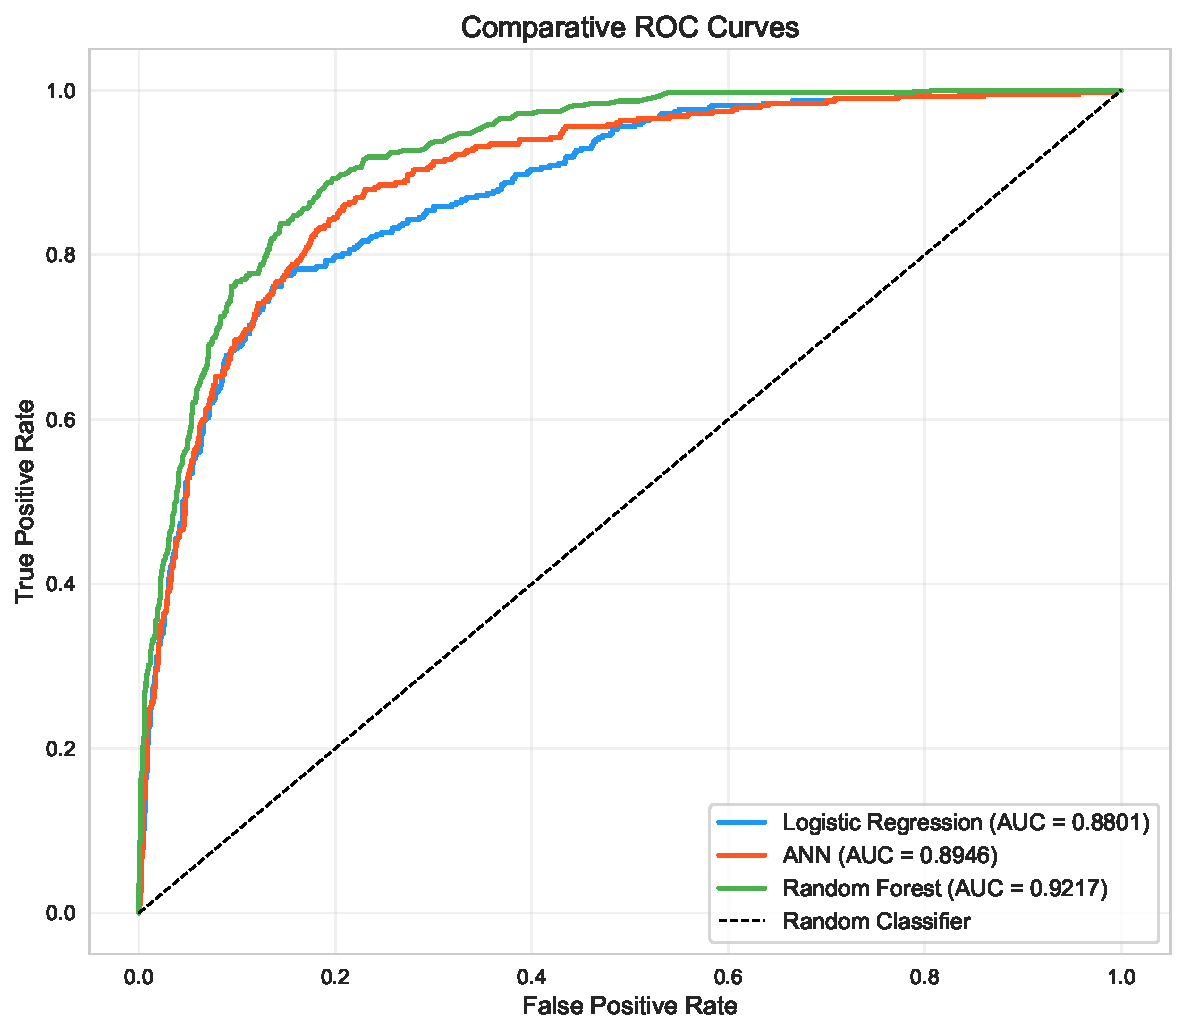
\includegraphics[width=0.65\textwidth]{comparative_roc.pdf}
    \caption{Comparative ROC curves.}
    \label{fig:roc_comp}
\end{figure}

\begin{figure}[H]
    \centering
    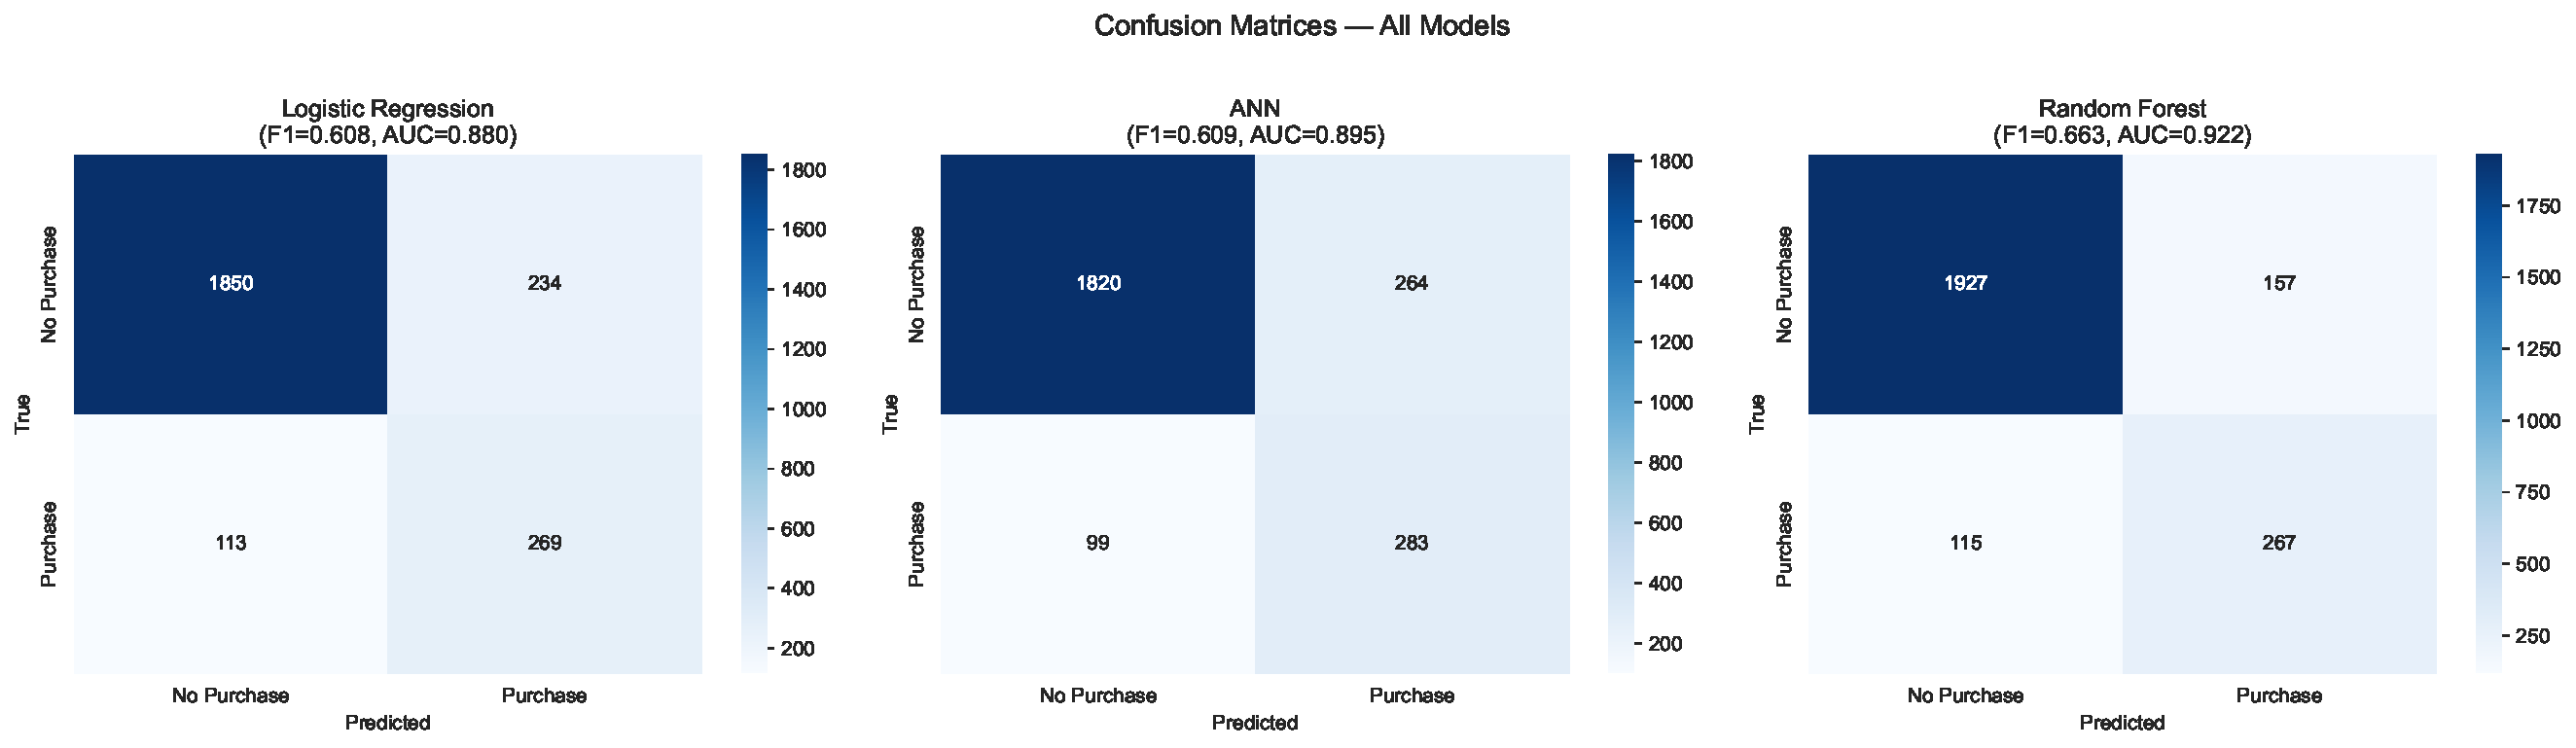
\includegraphics[width=\textwidth]{comparative_confusion_matrices.pdf}
    \caption{Confusion matrices for all three models on the test set (2,466 samples).}
    \label{fig:cm_comp}
\end{figure}

\subsection{Feature Importance via SHAP}

To unpack the decision-making process of the best-performing model, a SHAP (\textit{SHapley Additive exPlanations}) analysis was conducted on the Random Forest. As shown in Figure~\ref{fig:shap}, this method provides highly interpretable feature attributions, detailing both the magnitude and the direction of each variable's effect, a significant advantage over traditional Gini-based importance, which only reports absolute magnitude.

To properly interpret the SHAP beeswarm plot (Figure~\ref{fig:shap}a), three visual elements must be considered: the horizontal axis indicates the impact on the model's output (where positive SHAP values increase the likelihood of a purchase); the colour gradient represents the actual value of the feature for that specific session (red for high values, blue for low values); and the vertical thickness illustrates the density of data points sharing similar effects. 

Applying this reading key, the analysis highlights the following dynamics:

\begin{itemize}
    \item \textbf{PageValues} overwhelmingly acts as the dominant predictor; high values of this feature (red dots) consistently align on the positive side of the SHAP axis, strongly pushing the prediction towards a successful purchase.
    \item \textbf{Month} and \textbf{Administrative\_Duration} emerge as the second and third most influential features, indicating that the time of the year and the time spent on administrative pages hold a predictive power for this specific dataset.
    \item Conversely, high \textbf{ExitRates} and \textbf{BounceRates} act as strong negative signals. For these features, high values (red dots) are heavily concentrated on the negative side of the axis, driving the predictions towards the negative class (cart abandonment).
\end{itemize}

\begin{figure}[H]
    \centering
    \begin{subfigure}[t]{0.48\textwidth}
        \centering
        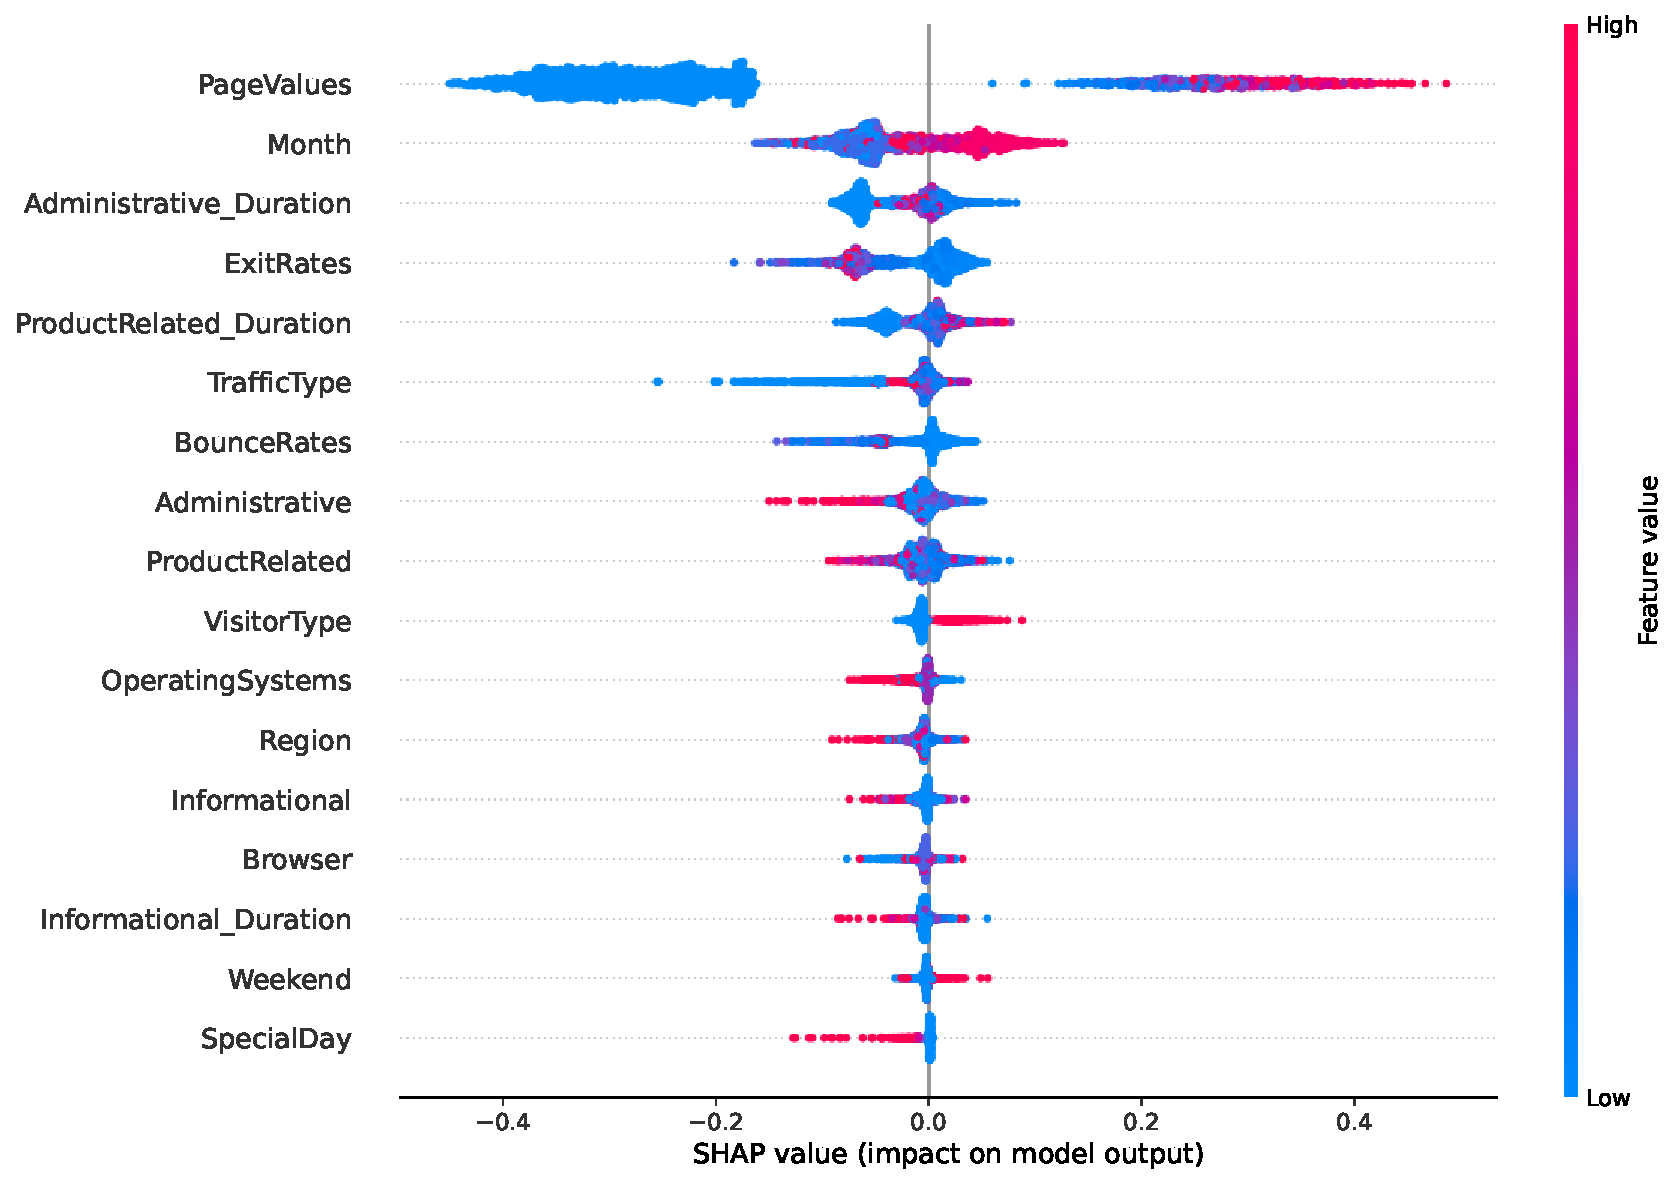
\includegraphics[width=\textwidth]{shap_beeswarm.pdf}
        \caption{Beeswarm: feature effect distributions.}
    \end{subfigure}
    \hfill
    \begin{subfigure}[t]{0.48\textwidth}
        \centering
        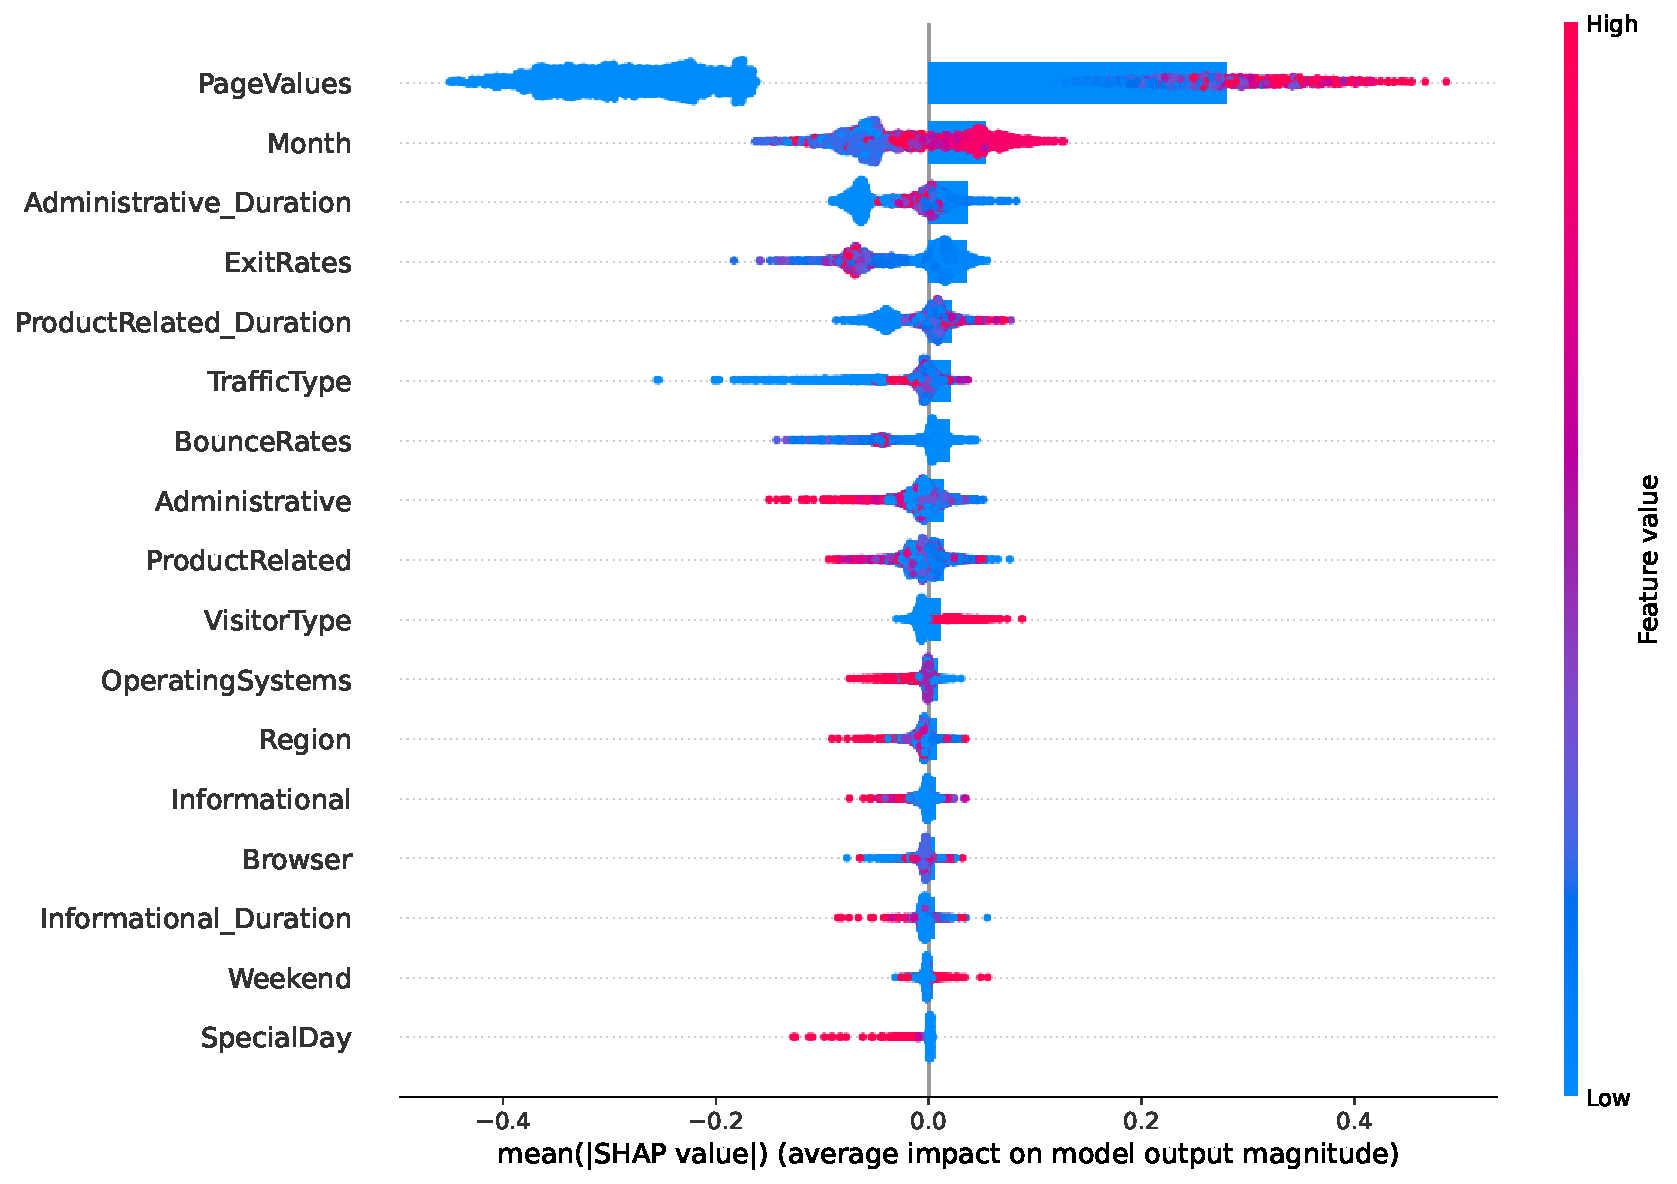
\includegraphics[width=\textwidth]{shap_bar.pdf}
        \caption{Bar plot: mean $|\text{SHAP}|$ feature ranking.}
    \end{subfigure}
    \caption{SHAP analysis of the Random Forest model on the test set.}
    \label{fig:shap}
\end{figure}
\section{Discussion and Conclusions}

\subsection{Discussion}

The experimental results demonstrate that the \textbf{Random Forest} outperforms both alternative architectures across all primary metrics. The key findings of this comparative study can be summarised as follows:

\begin{itemize}
    \item \textbf{Ensemble superiority}: The Random Forest achieved the best overall performance (ROC-AUC = 0.922, F1-Score = 0.663). This confirms that ensemble tree-based methods remain highly effective and are often the state-of-the-art choice for structured, tabular datasets~\cite{grinsztajn2022}.
    
    \item \textbf{Sensitivity of Deep Learning}: The ANN demonstrated the highest sensitivity, yielding the highest recall (0.741). This indicates its superior ability to capture the largest share of actual purchasers, but at the cost of lower precision (0.517). From a business perspective, this trade-off is highly valuable in scenarios where the opportunity cost of missing a potential buyer significantly outweighs the cost of a false positive (e.g., sending an unnecessary discount code).
    
    \item \textbf{Baseline competitiveness}: The Logistic Regression model proved remarkably competitive, achieving a ROC-AUC of 0.880 and an F1-Score of 0.608, which is only fractionally below the ANN's performance (0.609). This proximity suggests that the underlying decision boundary separating purchasers from non-purchasers is largely linear.
    
    \item \textbf{Impact of data balancing}: The rigorous management of class imbalance proved essential to the study's success. The application of SMOTE exclusively to the training set, coupled with class-weighted loss functions, empowered all models to achieve a meaningful minority-class recall despite the low 15.5\% baseline prevalence.
\end{itemize}

Furthermore, the SHAP analysis confirmed \textbf{PageValues} as the overwhelmingly dominant predictor. This provides a highly actionable business insight: improving page content to enhance perceived value, alongside reducing friction that leads to high bounce rates, represent the most effective strategic levers for conversion optimisation.

\subsection{Limitations}

While the study provides robust insights, certain limitations must be acknowledged. First, no systematic hyperparameter optimisation was performed, meaning the models' performances might not reflect their absolute theoretical maximum. Second, the implemented ANN architecture (128 $\rightarrow$ 64) is relatively shallow. Finally, the dataset originates from a single, anonymous e-commerce platform over a specific timeframe, implying that the identified behavioural patterns may not seamlessly generalise to different retail domains or contemporary browsing habits.

\subsection{Conclusions}

This study compared three distinct machine learning paradigms to predict e-commerce purchase intentions on a highly imbalanced dataset. While the Random Forest achieved the highest predictive performance and offered excellent SHAP-based interpretability, the comparative analysis revealed a crucial insight regarding model complexity.

The highly competitive performance of the Logistic Regression baseline (F1 = 0.608) compared to the Artificial Neural Network (F1 = 0.609) clearly illustrates the principle of \textbf{Occam's Razor}. Given that the simple linear model performs almost identically to the deep learning architecture, it is evident that much of the predictive signal in this dataset is linearly separable. Consequently, deploying a computationally expensive, "black-box" ANN provides negligible business value in this specific context.

Ultimately, the choice of the optimal model depends on the specific business objective. If the goal is to maximise overall accuracy and extract complex feature insights, the Random Forest is the superior choice. If the priority is to strictly minimise missed conversions, a high-recall setup is preferable. However, if computational efficiency, deployment speed, and strict interpretability are paramount, the Logistic Regression remains an exceptionally robust and pragmatic solution.
\begin{thebibliography}{9}

\bibitem{sakar2019}
Sakar, C.O., Polat, S.O., Katircioglu, M., \& Kastro, Y. (2019).
\textit{Real-time prediction of online shoppers' purchasing intention using multi-layer perceptron and LSTM recurrent neural networks}.
Neural Computing and Applications, 31(10), 6893--6908.

\bibitem{chawla2002}
Chawla, N.V., Bowyer, K.W., Hall, L.O., \& Kegelmeyer, W.P. (2002).
\textit{SMOTE: Synthetic Minority Over-sampling Technique}.
Journal of Artificial Intelligence Research, 16, 321--357.

\bibitem{lundberg2017}
Lundberg, S.M. \& Lee, S.I. (2017).
\textit{A Unified Approach to Interpreting Model Predictions}.
Advances in Neural Information Processing Systems (NeurIPS), 30.

\bibitem{breiman2001}
Breiman, L. (2001).
\textit{Random Forests}.
Machine Learning, 45(1), 5--32.

\bibitem{goodfellow2016}
Goodfellow, I., Bengio, Y., \& Courville, A. (2016).
\textit{Deep Learning}.
MIT Press.

\bibitem{grinsztajn2022}
Grinsztajn, L., Oyallon, E., \& Varoquaux, G. (2022).
\textit{Why do tree-based models still outperform deep learning on typical tabular data?}
Advances in Neural Information Processing Systems (NeurIPS), 35.

\end{thebibliography}



\end{document}